\chapter{Resultados}
Este cap\'itulo apresenta os resultados obtidos para cada uma das doze configura\c{c}\~oes investigadas.

\section{Resultados obtidos}
As figuras a seguir s\~ao o \textit{bloxplot} de cada configura\c{c}\~ao. A nomeclatura utilizada foi a seguinte: uma configura\c{c}\~ao \textbf{5-global-decay} significa:
\begin{itemize}
	\item \textbf{Cinco} part\'iculas no enxame
	\item Topologia \textbf{global}
	\item $\omega = 0,9 \rightarrow 0,4$
\end{itemize}
J\'a uma configura\c{c}\~ao \textbf{20-local-c1c2} significa:
\begin{itemize}
	\item \textbf{Vinte} part\'iculas no enxame
	\item Topologia \textbf{local}
	\item $C_1 = 2,5 \rightarrow 1,5$ e $C_2 = 1,5 \rightarrow 2,5$
\end{itemize}

\begin{figure}[H]
	\centering
	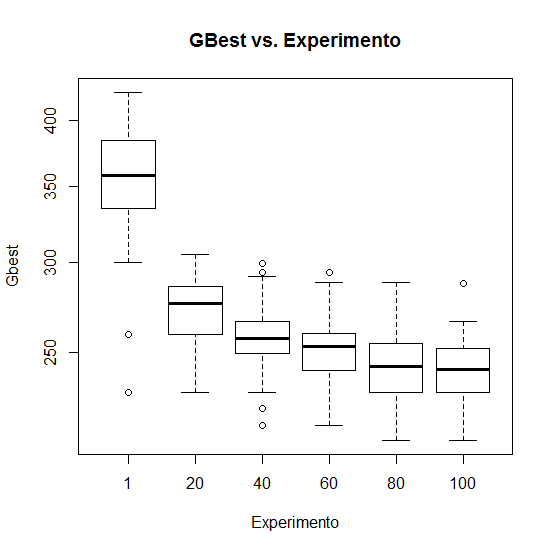
\includegraphics[width=.6\textwidth]{img/result_5_global_decay.png}
	\caption{Boxplot para configura\c{c}\~ao 5-global-decay}
	\label{fig:result_5_global_decay}
\end{figure}

\begin{figure}[H]
	\centering
	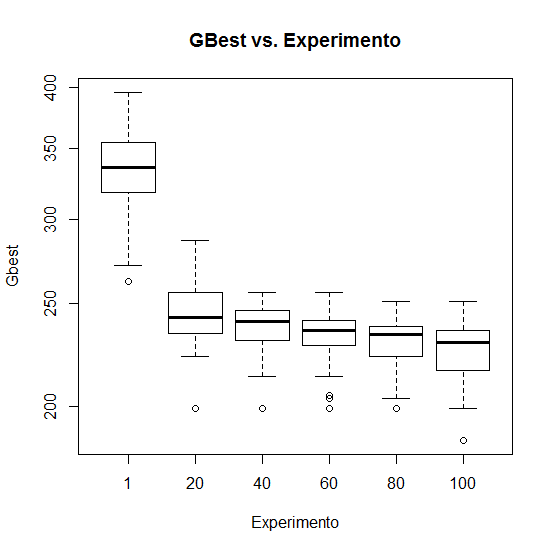
\includegraphics[width=.6\textwidth]{img/result_5_global_c1c2.png}
	\caption{Boxplot para configura\c{c}\~ao 5-global-c1c2}
	\label{fig:result_5_global_c1c2}
\end{figure}

\begin{figure}[H]
	\centering
	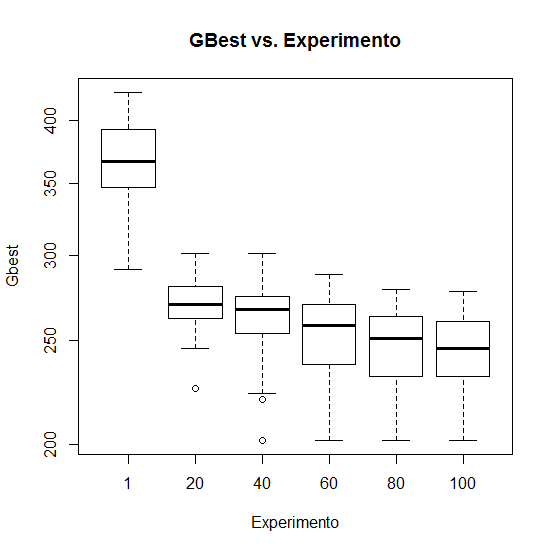
\includegraphics[width=.6\textwidth]{img/result_5_local_decay.png}
	\caption{Boxplot para configura\c{c}\~ao 5-local-decay}
	\label{fig:result_5_local_decay}
\end{figure}

\begin{figure}[H]
	\centering
	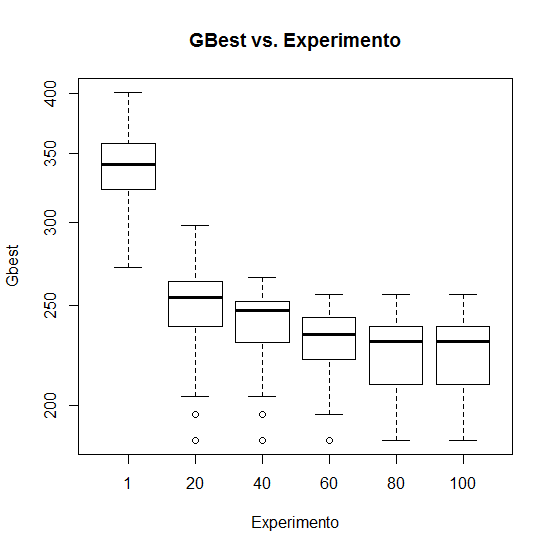
\includegraphics[width=.6\textwidth]{img/result_5_local_c1c2.png}
	\caption{Boxplot para configura\c{c}\~ao 5-local-c1c2}
	\label{fig:result_5_local_c1c2}
\end{figure}

\begin{figure}[H]
	\centering
	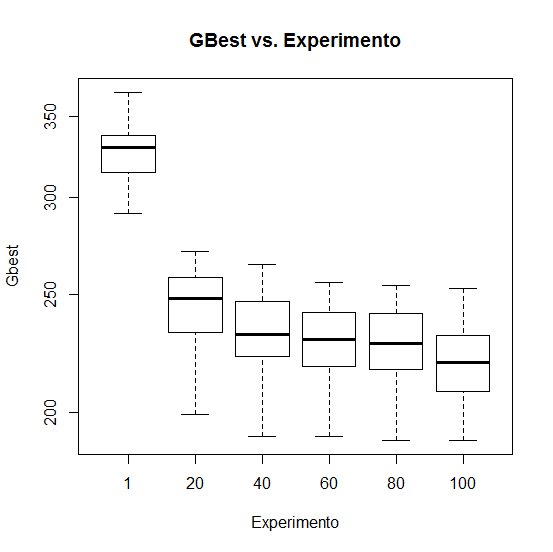
\includegraphics[width=.6\textwidth]{img/result_20_global_decay.png}
	\caption{Boxplot para configura\c{c}\~ao 20-global-decay}
	\label{fig:result_20_global_decay}
\end{figure}

\begin{figure}[H]
	\centering
	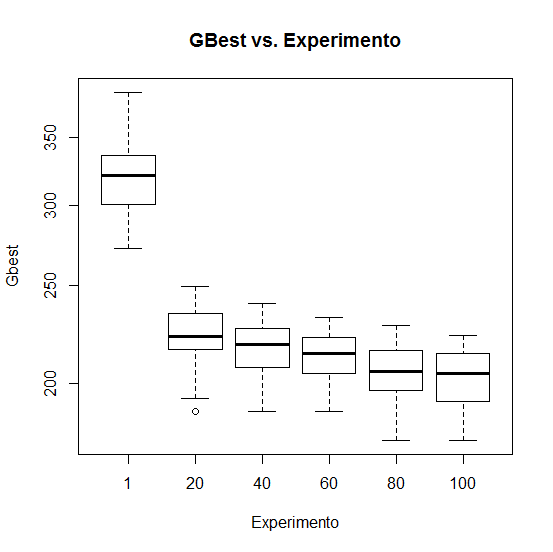
\includegraphics[width=.6\textwidth]{img/result_20_global_c1c2.png}
	\caption{Boxplot para configura\c{c}\~ao 20-global-c1c2}
	\label{fig:result_20_global_c1c2}
\end{figure}

\begin{figure}[H]
	\centering
	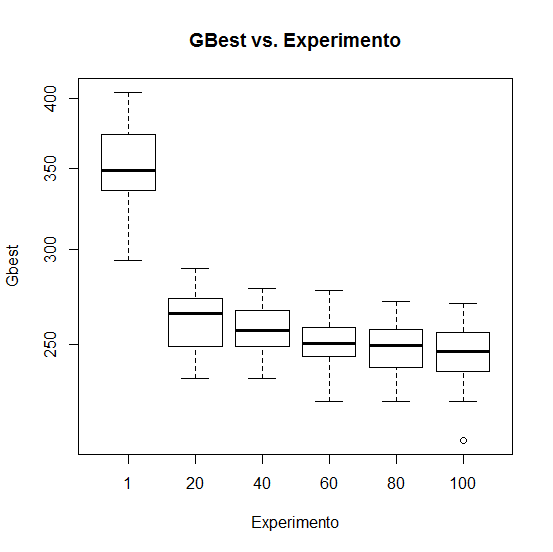
\includegraphics[width=.6\textwidth]{img/result_20_local_decay.png}
	\caption{Boxplot para configura\c{c}\~ao 20-local-decay}
	\label{fig:result_20_local_decay}
\end{figure}

\begin{figure}[H]
	\centering
	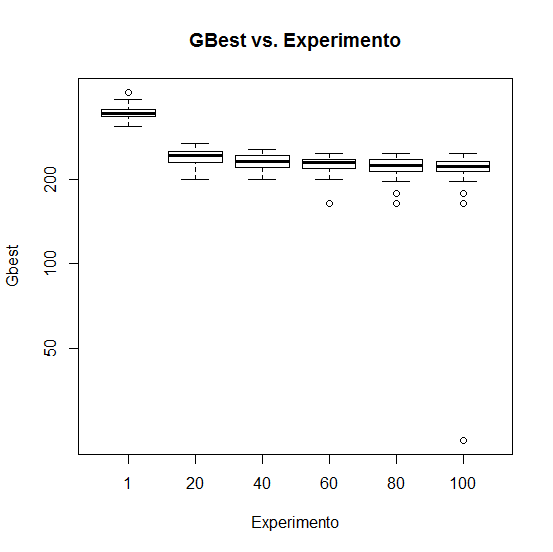
\includegraphics[width=.6\textwidth]{img/result_20_local_c1c2.png}
	\caption{Boxplot para configura\c{c}\~ao 20-local-c1c2}
	\label{fig:result_20_local_c1c2}
\end{figure}

\begin{figure}[H]
	\centering
	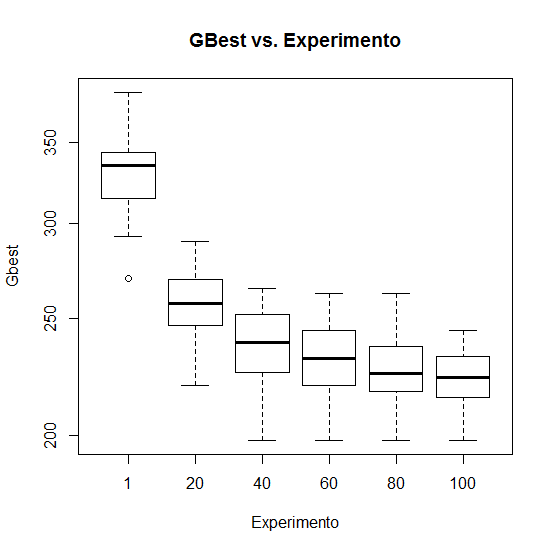
\includegraphics[width=.6\textwidth]{img/result_50_global_decay.png}
	\caption{Boxplot para configura\c{c}\~ao 50-global-decay}
	\label{fig:result_50_global_decay}
\end{figure}

\begin{figure}[H]
	\centering
	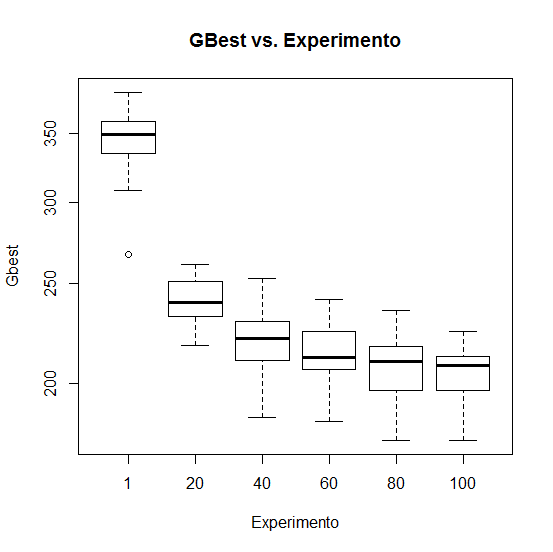
\includegraphics[width=.6\textwidth]{img/result_50_global_c1c2.png}
	\caption{Boxplot para configura\c{c}\~ao 50-global-c1c2}
	\label{fig:result_50_global_c1c2}
\end{figure}

\begin{figure}[H]
	\centering
	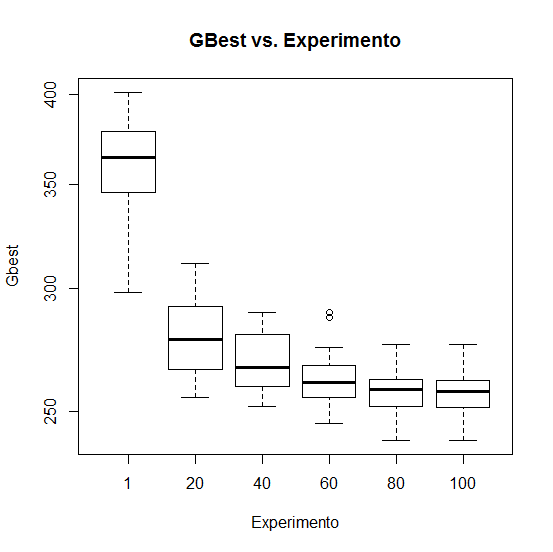
\includegraphics[width=.6\textwidth]{img/result_50_local_decay.png}
	\caption{Boxplot para configura\c{c}\~ao 50-local-decay}
	\label{fig:result_50_local_decay}
\end{figure}

\begin{figure}[H]
	\centering
	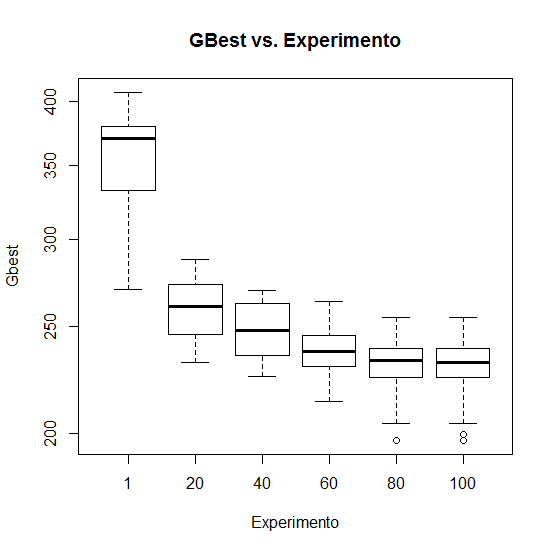
\includegraphics[width=.6\textwidth]{img/result_50_local_c1c2.png}
	\caption{Boxplot para configura\c{c}\~ao 50-local-c1c2}
	\label{fig:result_50_local_c1c2}
\end{figure}


\section{Compara\c{c}\~ao de execu\c{c}\~ao}
Ap\'os estes experimentos serem executados foi realizado o teste de Wilcoxon Pareado com 95\% de intervalo de confian\c{c}a. O resultado est\'a na Tabela \ref{tab:teste_wilcoxon}.
\begin{table}[H]
	\centering
	\caption{Teste de Wilcoxon Pareado para varia\c{c}\~ao nos par\^ametros $C_1$ e $C_2$}
	\begin{tabular}{|c|c|c|c|}
		\hline
		                    & 5 part\'iculas & 20 part\'iculas & 50 part\'iculas \\ \hline
		5 part\'iculas      & -              & P               & P \\
		20 part\'iculas     & M              & -               & P \\
		50 part\'iculas     & M              & M               & - \\
		\hline
	\end{tabular}
	\label{tab:teste_wilcoxon}
\end{table}